\section{Numerical Methods Details}
\label{app:numerical-methods-details}
This appendix supplies the numerical-method detail behind
Section~\ref{subsubsec:cross-sectional-reduction-selected-1d-model} and the
comparison operator in
Section~\ref{subsec:plane-tetrahedron-comparison-operator}. It is supporting
method detail, not a claim of external-solver parity for the implemented solver.
The continuous identities are read under
Convention~\ref{conv:foundation-standing-regularity}; computed quantities are
read through the following numerical-record convention.

\begin{convention}[Computed realization record]
\label{conv:computed-realization-record}
A computed realization is interpreted only through the model, closure,
discretization, grid, timestep policy, boundary-state rule, output operator,
and diagnostic metadata recorded for that realization. Symbols such as
$D_t$, $D_z$, numerical fluxes, residual arrays, and sampled norms denote
recorded discrete objects unless a section explicitly switches back to a
continuum identity.
\end{convention}

The time interval, output rectangle, and norm notation follow
Definition~\ref{def:foundation-time-and-compact-set-notation} and
Definition~\ref{def:foundation-norm-conventions}; discrete residuals use the
recorded $D_t$, $D_z$, grid, and quadrature weights rather than unnamed
continuum derivatives.

\subsection{Implemented secondary solver surfaces}
\label{app:num-secondary-solver-surfaces}

The principal C23/C40 comparison uses MUSCL finite volume with minmod limiting
and native SSPRK3. Table~\ref{tab:implemented-discretization-surface} records
the wider implemented surface so that benchmark and sensitivity rows can be
interpreted without moving secondary methods into the main methodology
narrative.

\begin{table}[!htb]
    \centering
    \scriptsize
    \caption{Implemented discretization surface used by the report. The principal
    comparison in this report uses MUSCL finite volume with minmod limiting and
    native SSPRK3; the other entries are benchmark, sensitivity, or backend
    parity context supported by the local Julia project.}
    \label{tab:implemented-discretization-surface}
    \begin{tabularx}{\textwidth}{@{}
        >{\raggedright\arraybackslash}p{0.20\textwidth}
        >{\raggedright\arraybackslash}p{0.30\textwidth}
        >{\raggedright\arraybackslash}X@{}}
        \toprule
        \textbf{Surface} & \textbf{Implemented option} & \textbf{Report role} \\
        \midrule
        Spatial
            & First-order finite-volume Rusanov
            & Low-order cell-average baseline and DG $p=0$ bridge. \\
        Spatial
            & MUSCL finite volume with minmod-limited interface states and
            Rusanov flux
            & Principal C23/C40 comparison method and main empirical
            refinement target. \\
        Spatial
            & Characteristic WENO3 finite volume with Rusanov flux
            & Opt-in native finite-volume implementation check and smooth-regime
            sensitivity method; not the principal comparison method. \\
        Spatial
            & Richtmyer/Lax--Wendroff finite volume with minmod-limited
            interface states
            & Native fixed-step sensitivity method; not exposed through the
            SciML \texttt{ODEProblem} backend because its flux predictor depends
            on $\Delta t/\Delta z$. \\
        Spatial
            & Modal Legendre DG implemented for degrees $p=0,\ldots,4$
            & Secondary native-DG surface. Descriptor-health and
            package-benchmark rows may currently exercise only $p=0,1,2$;
            the p-refinement verification workflow runs through $p=4$. These
            rows are appendix context, not the principal C23/C40 comparison
            method. \\
        Time
            & Forward Euler, SSPRK2, SSPRK3, and SSPRK54
            & Native fixed-step options; SSPRK3 is the selected reported
            integrator, while Euler, SSPRK2, and SSPRK54 are diagnostic or
            higher-order sensitivity rows. \\
        Time
            & SciML/OrdinaryDiffEq \texttt{auto}, \texttt{tsit5},
            \texttt{vern7}, \texttt{vern9}, and \texttt{rodas5p}
            & Adaptive backend-parity checks for semi-discrete operators that
            the current \texttt{ODEProblem} path supports. \\
        \bottomrule
    \end{tabularx}
\end{table}


\subsection{Secondary implementation-health records}
\label{app:num-secondary-implementation-health}
\label{subsec:verification-reproducibility}
\label{subsec:package-benchmark-suite}

The package benchmark suite records implementation-health stages for the Julia
solver: descriptor health, sampled self-convergence, native/SciML
cross-integrator discrepancy, stationary-Stokes projection rows,
rheology/profile sensitivity, OpenBF-style boundary handling, and
resolved-velocity output diagnostics. These records check that documented solver
surfaces remain runnable and that generated report assets retain their expected
columns. They are not the principal C23/C40 comparison method, and they do not
supersede the MMS or geometry-rest evidence in Chapter~\ref{sec:numerical-verification}.

\IfFileExists{figures/static/static/tables/package-benchmark/package-benchmark-summary.tex}{%
    \begin{table}[!htb]
    \centering
    \scriptsize
    \caption{Benchmark stage summary.}
    \begin{tabular}{@{}lrrr@{}}
        \toprule
        Stage & Rows & OK & Skipped/error \\
        \midrule
        case results & 18 & 18 & 0 \\
        refinement & 128 & 128 & 0 \\
        backend parity & 18 & 18 & 0 \\
        stokes ic & 12 & 12 & 0 \\
        rheology profile & 60 & 60 & 0 \\
        boundary openbf & 3 & 3 & 0 \\
        resolved3d & 4 & 4 & 0 \\
        \bottomrule
    \end{tabular}
\end{table}

}{%
    \begin{center}
    \small
    \emph{Benchmark table fragment unavailable in this checkout. Run the
    benchmark renderer to populate
    \path{figures/static/static/tables/package-benchmark/}.}
    \end{center}
}

\subsubsection{Nonselected DG p/h demonstration}

The manufactured-solution p/h demonstration is a secondary smooth-solution
implementation check for the native modal-DG surface. The implemented DG support
runs through $p=4$, while descriptor-health or package-benchmark rows may use
only selected degrees such as $p=0,1,2$. These rows are appendix context, not the
principal MUSCL/Rusanov/SSPRK3 comparison method.

\IfFileExists{figures/static/static/tables/verification/p_h_refinement_demo.tex}{%
    \begin{table}[!htb]
    \centering
    \scriptsize
    \caption{Manufactured-solution p- and h-refinement demonstration. The h-refinement rows report observed order from adjacent grid spacings; the p-refinement rows report error reduction relative to the previous polynomial degree.}
    \resizebox{\textwidth}{!}{%
    \begin{tabular}{@{}lrrrrrrrrr@{}}
        \toprule
        Sweep & $p$ & $N$ & DOFs & $\|e_a\|_2$ & h-order & p-reduction & $\|e_q\|_2$ & h-order & p-reduction \\
        \midrule
        h-refinement & 2 & 20 & 120 & 9.797e-06 & 1.457 & -- & 0.009629 & 1.052 & -- \\
        h-refinement & 2 & 40 & 240 & 3.569e-06 & 1.488 & -- & 0.004643 & 1.209 & -- \\
        h-refinement & 2 & 80 & 480 & 1.272e-06 & 1.51 & -- & 0.002009 & 1.424 & -- \\
        h-refinement & 2 & 160 & 960 & 4.467e-07 & -- & -- & 7.489e-04 & -- & -- \\
        p-refinement & 0 & 40 & 80 & 1.078e-05 & -- & -- & 0.002585 & -- & -- \\
        p-refinement & 1 & 40 & 160 & 3.569e-06 & -- & 3.022 & 0.004645 & -- & 0.5565 \\
        p-refinement & 2 & 40 & 240 & 3.569e-06 & -- & 1 & 0.004643 & -- & 1 \\
        p-refinement & 3 & 40 & 320 & 3.569e-06 & -- & 0.9999 & 0.004643 & -- & 1 \\
        p-refinement & 4 & 40 & 400 & 3.569e-06 & -- & 1 & 0.004642 & -- & 1 \\
        \bottomrule
    \end{tabular}%
    }
\end{table}

}{%
    \begin{center}
    \small
    \emph{p/h-refinement table unavailable in this checkout. Run
    \texttt{verify ph-refinement} and the renderer to populate
    \path{figures/static/static/tables/verification/}.}
    \end{center}
}

\begin{figure}[!htb]
    \centering
    \IfFileExists{figures/static/static/rendered/p-h-refinement-demo.pdf}{%
        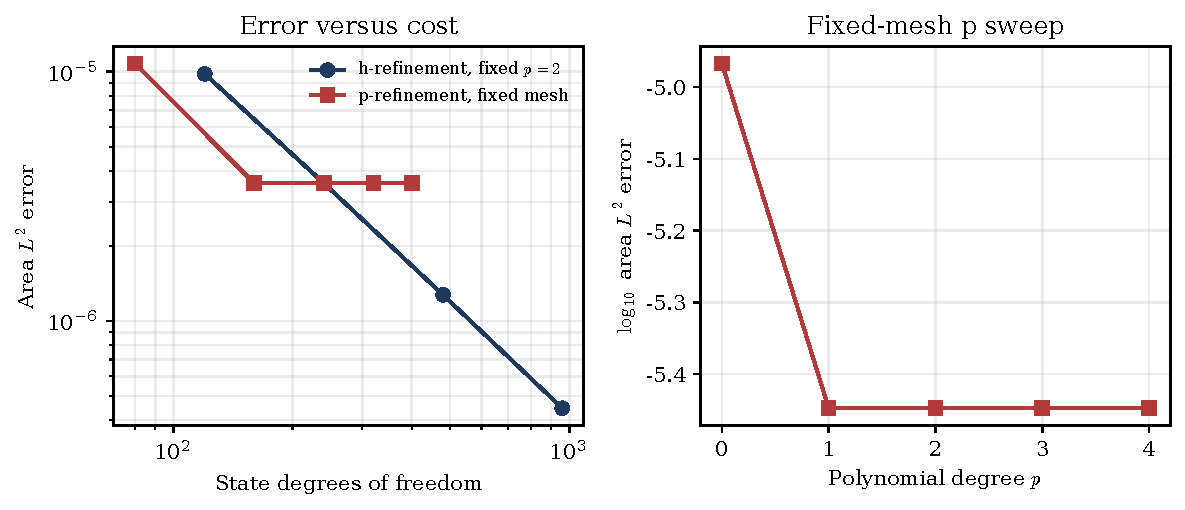
\includegraphics[width=0.92\linewidth]{figures/static/static/rendered/p-h-refinement-demo.pdf}
    }{%
        \fbox{\parbox{0.82\linewidth}{\centering p/h-refinement demonstration
        asset unavailable in this checkout.}}
    }
    \caption{Manufactured-solution p- and h-refinement demonstration for the
    modal DG surface. The comparison isolates fixed-degree h-refinement from a
    fixed-mesh p sweep and should be interpreted as smooth-case implementation
    evidence, not physical validation.}
    \label{fig:ph-refinement-demo}
\end{figure}

\subsubsection{Self-convergence and cross-integrator records}
\label{subsec:sampled-self-convergence}

Self-convergence and backend-parity rows are empirical implementation-health
checks. They can reveal grid sensitivity, boundedness problems, or
integration-policy discrepancies, but they do not replace the exact-solution MMS
rows and do not establish stability of the nonlinear semi-discrete operator.

\begin{figure}[!htb]
    \centering
    \IfFileExists{figures/static/static/rendered/package-benchmark-convergence.pdf}{%
        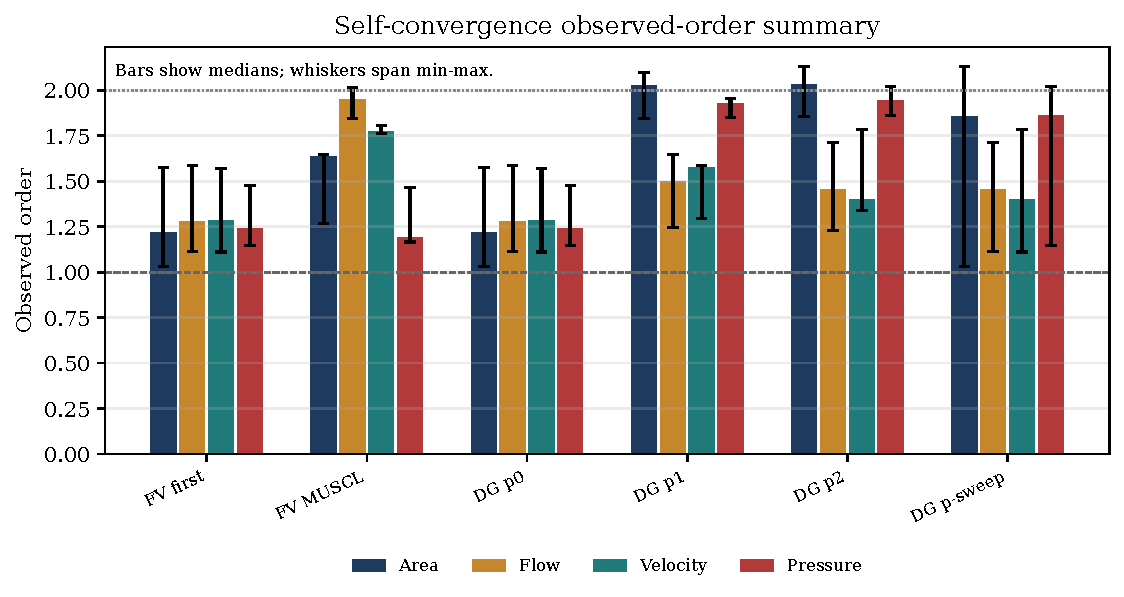
\includegraphics[width=0.86\linewidth]{figures/static/static/rendered/package-benchmark-convergence.pdf}
    }{%
        \fbox{\parbox{0.82\linewidth}{\centering Benchmark convergence
        asset unavailable in this checkout.}}
    }
    \caption{Self-convergence observed-order summary reported by the benchmark
    renderer. This is a sampled implementation-check diagnostic; the MMS table in
    Section~\ref{subsec:mms-verification} is the stronger exact-solution
    verification evidence.}
    \label{fig:package-benchmark-convergence}
\end{figure}

\begin{figure}[!htb]
    \centering
    \IfFileExists{figures/static/static/rendered/package-benchmark-backend-parity.pdf}{%
        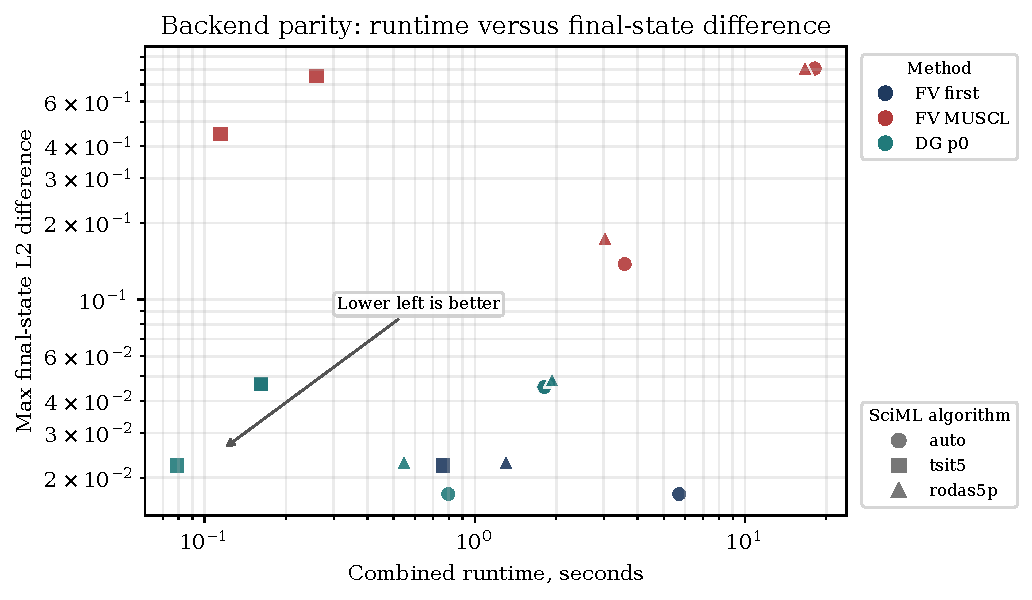
\includegraphics[width=0.86\linewidth]{figures/static/static/rendered/package-benchmark-backend-parity.pdf}
    }{%
        \fbox{\parbox{0.82\linewidth}{\centering Benchmark
        cross-integrator discrepancy asset unavailable in this checkout.}}
    }
    \caption{Native/SciML cross-integrator discrepancy versus runtime for
    compatible methods. The native path uses the stagewise positivity limiter;
    the SciML path integrates the unprojected semi-discrete system. The figure
    is therefore a cross-integrator diagnostic, not a proof of solver equivalence.}
    \label{fig:package-benchmark-backend-parity}
\end{figure}

\subsubsection{Resolved-velocity and descriptor sensitivity benchmark records}
\label{subsec:resolved-velocity-benchmark-diagnostic}

The package benchmark also keeps a resolved-velocity output-operator stage. Its
role here is limited: it checks that the \texttt{CrossSectionQuadratureOperator}
report path remains executable and records the same kind of mean absolute
velocity discrepancy used in Section~\ref{sec:resolved-3d-comparison}. The
detailed interpretation of the resolved comparison belongs to
Chapter~\ref{sec:resolved-3d-comparison}.

\begin{figure}[!htb]
    \centering
    \IfFileExists{figures/static/static/rendered/package-benchmark-resolved3d.pdf}{%
        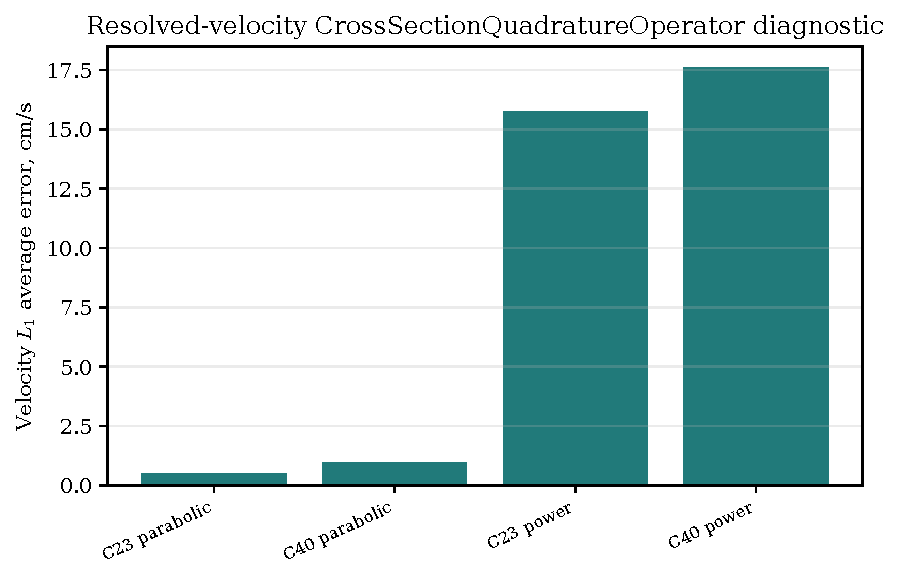
\includegraphics[width=0.72\linewidth]{figures/static/static/rendered/package-benchmark-resolved3d.pdf}
    }{%
        \fbox{\parbox{0.82\linewidth}{\centering Benchmark
        resolved-velocity diagnostic asset unavailable in this checkout.}}
    }
    \captionsetup{justification=raggedright,singlelinecheck=false}
    \caption{Resolved-velocity output-operator diagnostic summary for the
    available local cases. The rendered value is the section-wise mean absolute
    velocity discrepancy for the declared
    \texttt{CrossSectionQuadratureOperator}.}
    \label{fig:package-benchmark-resolved3d}
\end{figure}

\subsubsection{Descriptor sensitivity records}
\label{subsec:verification-sensitivity-checks}

The rheology/profile benchmark stage is a descriptor-level sensitivity check. It
is retained to show that the descriptor options remain connected to the
benchmark record, but it is not used to support the principal C23/C40 comparison
claim.

\begin{figure}[!htb]
    \centering
    \IfFileExists{figures/static/static/rendered/package-benchmark-rheology-profile.pdf}{%
        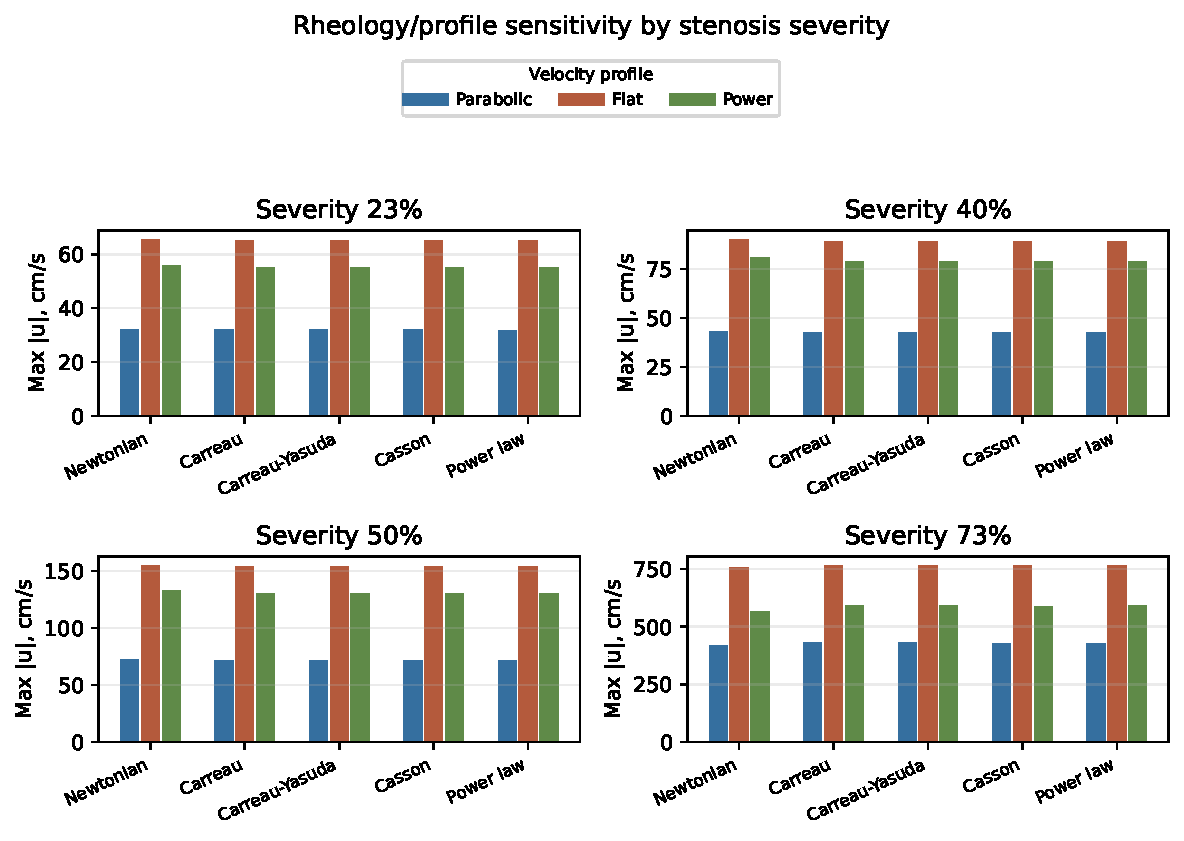
\includegraphics[width=0.86\linewidth]{figures/static/static/rendered/package-benchmark-rheology-profile.pdf}
    }{%
        \fbox{\parbox{0.82\linewidth}{\centering Benchmark
        rheology/profile asset unavailable in this checkout.}}
    }
    \caption{Rheology/profile sensitivity summary for declared descriptor
    combinations. This stage checks descriptor response direction; it is not
    part of the principal C23/C40 comparison evidence.}
    \label{fig:package-benchmark-rheology-profile}
\end{figure}


\subsection{Fixed-wall stationary-Stokes refinement record}
\label{app:num-stationary-stokes-refinement}
\label{subsec:stationary-stokes-projection-checks}

The local three-dimensional refinement study is limited to a fixed-wall
stationary-Stokes problem on the smooth idealized stenosis geometry. The public
entrypoint \path{run_stationary_stokes_refinement} constructs generated Gridap
tetrahedral meshes from the same $C^\infty$ radius profile used by the reduced
model, solves a pressure-drop-driven stationary Stokes problem, evaluates
section-averaged velocity and pressure from the finite-element field, and
compares those averages with the resistance/projection quantities used by the
stationary-Stokes initializer. This keeps the initializer behavior unchanged:
the study is an additional diagnostic record, not a replacement for the 1D
initial-condition contract.

For a Newtonian fixed-wall Stokes field, the sampled stress and wall-traction
diagnostics use
\begin{flalign*}
    \quad
    \boldsymbol\sigma(\vu,p)
    &=
    -p\mathbf I+\mu\left(\nabla\vu+\nabla\vu^\top\right), &&
    \mu=\rho\nu,\\
    \quad
    \mathbf t_w
    &=
    \boldsymbol\sigma\mathbf n, &
    \boldsymbol\tau_w
    &=
    \mathbf t_w-(\mathbf t_w\cdot\mathbf n)\mathbf n. &&
\end{flalign*}
Here $\mathbf n$ is the analytic outward normal of the $C^\infty$ wall profile.
The reported means and maxima are fixed-wall fluid-stress diagnostics sampled
from the finite-element solution. They are not structural displacement, wall
velocity, structural stress, or resolved FSI interface-work outputs.


\IfFileExists{figures/static/static/tables/verification/stationary_stokes_refinement.tex}{%
    \begin{table}[!htb]
    \centering
    \scriptsize
    \caption{Stationary-Stokes projection and mesh-refinement diagnostics.}
    \begin{tabular}{@{}lrrrrrr@{}}
        \toprule
        Case & Nodes & Cells & $\langle Q\rangle$ & FE--proj. $u$ & Finest $u$ & WSS max \\
        \midrule
stokes-s23-8x2x8 & 153 & 576 & 0.1743 & 0.2012 & 0.3643 & 5.644 \\
stokes-s23-16x4x16 & 1105 & 5376 & 0.1743 & 0.1928 & 0.000e+00 & 8.446 \\
stokes-s40-8x2x8 & 153 & 576 & 0.1286 & 0.378 & 0.5212 & 6.034 \\
stokes-s40-16x4x16 & 1105 & 5376 & 0.1286 & 0.2201 & 0.000e+00 & 11.06 \\
        \bottomrule
    \end{tabular}
\end{table}

}{%
    \begin{center}
    \small
    \emph{Stationary-Stokes refinement table unavailable in this checkout. Run
    the stationary-Stokes refinement workflow to populate the verification
    table.}
    \end{center}
}

\subsection{Elastic-potential balance-law form}
\label{app:num-elastic-potential-form}

The reduced state is $\mathbf U=(A,Q)^\top$. For a member of the
$\mathcal W_{\mathrm{elastic1D}}$ balance-law contract with prescribed
momentum-flux correction $\alpha$, the reference elastic-potential form is
\begin{flalign*}
    \quad
    \pd_t A+\pd_z Q &=0, &&\\
    \quad
    \pd_t Q
    +
    \pd_z \left(\alpha\frac{Q^2}{A}+\Psi(A,z,t)\right)
    &=
    S_{\mathrm{geom}}(A,z,t)
    -
    C_f(z,A,Q)\frac{Q}{A}. &&
\end{flalign*}
The elastic potential satisfies
\begin{flalign*}
    \quad
    \pd_A \Psi(A,z,t)
    =
    \frac{A}{\rho} \pd_A p_{\mathrm g}(A,z,t), &&
\end{flalign*}
and the geometry source is
\begin{flalign*}
    \quad
    S_{\mathrm{geom}}(A,z,t)
    =
    \left.\pd_z \Psi(A,z,t)\right|_A
    -
    \frac{A}{\rho}
    \left.\pd_z p_{\mathrm g}(A,z,t)\right|_A. &&
\end{flalign*}
For the selected Canic--Koiter wall-law member, assuming
$p_{\mathrm{ext}}$ is independent of $A$,
\begin{flalign*}
    \quad
    c^2(A,z)
    =
    \frac{A}{\rho} \pd_A p_{\mathrm g}(A,z,t)
    =
    \frac{\beta(z)\sqrt A}{2\rho A_0(z)}. &&
\end{flalign*}
Under the selected solver-coordinate map $A=\pi a$ and
$A_0=\pi R_0^2$, the implemented member corresponds to
$\beta(z)=\sqrt{\pi}K R_0(z)^2/R_{\max}^2$. Therefore
\begin{flalign*}
    \quad
    c^2(a,z)
    =
    \frac{K}{2\rho R_{\max}^2}\sqrt a
    &&
\end{flalign*}
for the evolution wall law used in the reported finite-volume runs.
Freeze $z$, the wall-closure data, and the source terms, and consider the
homogeneous $(A,Q)$ flux Jacobian associated with
$(Q,\alpha Q^2/A+\Psi(A,z,t))^\top$. On a positive-area state $A>0$, with
flow rate $Q$, mean velocity $Q/A$, prescribed momentum-flux correction
$\alpha$, and
$c^2(A,z)\defined(A/\rho)\pd_A p_{\mathrm g}(A,z,t)$, its eigenvalues are
\begin{flalign*}
    \quad
    \lambda_\pm(A,Q;z)
    =
    \alpha\frac{Q}{A}
    \pm
    \sqrt{c^2(A,z)+\alpha(\alpha-1)\left(\frac{Q}{A}\right)^2}. &&
\end{flalign*}
For the displayed elastic wall law, $c^2>0$ when $\beta>0$, $A>0$,
$A_0>0$, and $\rho>0$. Strict hyperbolicity of the homogeneous elastic
subsystem further requires the characteristic radicand
\begin{flalign*}
\quad
    c^2(A,z)+\alpha(\alpha-1)\left(\frac{Q}{A}\right)^2
    >0 &&
\end{flalign*}
to be positive on the reported state set. These speeds reduce to
$Q/A\pm c(A,z)$ in the special $\alpha=1$ reference case. The subcritical
case used in Assumption~\ref{ass:1d-subcritical-boundary-regime} is
$\lambda_-<0<\lambda_+$, so one characteristic enters through the inlet, one
characteristic enters through the outlet, and one scalar boundary condition is
imposed at each end of the vessel.
The displayed derivatives of $A_0$, $\beta$, $p_{\mathrm g}$, and
$\Psi$ are continuum notation for the model contract. A computed record may
realize them through explicitly recorded finite-difference or source-split
operators; changing that realization changes the computed map.

\subsection{Semi-discrete solver operator}
\label{app:num-current-solver-operator}

The implemented solver stores a radius-squared area coordinate in the variable
\texttt{A}. In this subsection write that coordinate as $a=R^2$. The
physical circular cross-sectional area is
$A_{\mathrm{phys}}=\pi a$. This is a solver-specific convention; the continuum
and classical 1D model sections keep $A$ for physical cross-sectional area.

For $N$ finite-volume cells, let
\begin{flalign*}
    \quad
    z_i=\left(i-\frac{1}{2}\right)\Delta z,\qquad
    \Delta z=\frac{L}{N},\qquad
    u_h(t)=
    \left(a_1(t),\ldots,a_N(t),q_1(t),\ldots,q_N(t)\right)^\top. &&
\end{flalign*}
The semi-discrete system exposed by \path{semidiscretize} and \path{rhs!} is
\begin{flalign*}
    \quad
    \dot u_h=\mathcal L_h(u_h,t;\theta), &&
\end{flalign*}
where $\theta$ denotes the recorded physical, geometry, grid, and solver
parameters. Componentwise,
\begin{flalign*}
    \quad
    \dot a_i
    &=
    -
    \frac{\widehat F^a_{i+1/2}-\widehat F^a_{i-1/2}}{\Delta z}, &&\\
    \quad
    \dot q_i
    &=
    -
    \frac{\widehat F^q_{i+1/2}-\widehat F^q_{i-1/2}}{\Delta z}
    +\widehat S_i. &&
\end{flalign*}
All divisions by $a$ use the positivity-regularized value of the
radius-squared area coordinate.

With $K=Eh/(1-\sigma^2)$, Canic conservative-form reference radius
$R_0^*=R_{\max}$, velocity-profile momentum factor
$\alpha_{\mathcal P}$, and
$\alpha_c(R_0')=-2(R_0')^2/35$, define
$\iota_{\mathcal M}=1$ for the \texttt{canic-extended-1d} forward-model
descriptor and $\iota_{\mathcal M}=0$ for
\texttt{classical-1d-no-slip}, the manifest token for the classical
parabolic-profile baseline. The semi-discrete full-state flux is
\begin{flalign*}
    \quad
    \mathbf F(a,q,z)
    =
    \left(
        q,\,
        \left(\alpha_{\mathcal P}+\iota_{\mathcal M}\alpha_c(R_0'(z))\right)\frac{q^2}{a}
        +\frac{K}{3\rho R_{\max}^2}a^{3/2}
    \right)^\top. &&
\end{flalign*}
At each interface,
\begin{flalign*}
    \quad
    \widehat{\mathbf F}_{i+1/2}
    =
    \frac{1}{2}\left[
        \mathbf F(\mathbf U^-_{i+1/2},z_{i+1/2})
        +
        \mathbf F(\mathbf U^+_{i+1/2},z_{i+1/2})
    \right]
    -
    \frac{1}{2}s_{i+1/2}
    \left(\mathbf U^+_{i+1/2}-\mathbf U^-_{i+1/2}\right), &&
\end{flalign*}
where $\mathbf U=(a,q)^\top$. The MUSCL finite-volume method limits the conservative
solver variables componentwise. For an interior cell,
\begin{flalign*}
    \quad
    \delta_i^a
    &=
    \operatorname{minmod}(a_i-a_{i-1},\,a_{i+1}-a_i),
    &
    \delta_i^q
    &=
    \operatorname{minmod}(q_i-q_{i-1},\,q_{i+1}-q_i), &&\\
    \quad
    \mathbf U^-_{i+1/2}
    &=
    (a_i+\tfrac12\delta_i^a,\,
     q_i+\tfrac12\delta_i^q)^\top,
    &
    \mathbf U^+_{i+1/2}
    &=
    (a_{i+1}-\tfrac12\delta_{i+1}^a,\,
     q_{i+1}-\tfrac12\delta_{i+1}^q)^\top. &&
\end{flalign*}
The active limiter is the two-argument minmod limiter, equivalent to the
$\theta=1$ member of the generalized minmod family. Boundary-adjacent cell
slopes are set to zero and paired with the ghost states described in
Appendix~\ref{app:num-boundary-state-realization}. Positivity limiting is
applied to reconstructed $a$ states before flux evaluation. The cell source is
not MUSCL-reconstructed; it is evaluated at cell centers using the recorded
$D_z^h$ differences below. The first-order finite-volume method is the separate
path that passes neighboring cell and ghost states directly to the same
Rusanov flux.

The implemented finite-volume surface also includes an opt-in characteristic
WENO3 reconstruction. At an interior interface $i+1/2$ with the four-cell
stencil $(i-1,i,i+1,i+2)$, the implementation freezes the homogeneous
flux-Jacobian eigenvalues at the local reference state
\begin{flalign*}
    \quad
    \mathbf U_{\mathrm{ref}}
    &=
    \frac{1}{2}(\mathbf U_i+\mathbf U_{i+1}) &&
\end{flalign*}
and projects conservative states into characteristic components
\begin{flalign*}
    \quad
    w^- &= \frac{\lambda^+ a-q}{\lambda^+-\lambda^-},
    &
    w^+ &= \frac{-\lambda^- a+q}{\lambda^+-\lambda^-}. &&
\end{flalign*}
For a scalar characteristic component with stencil values
$(v_{i-1},v_i,v_{i+1})$, the left state uses
\begin{flalign*}
    \quad
    p_0^- &= -\frac{1}{2}v_{i-1}+\frac{3}{2}v_i,
    &
    p_1^- &= \frac{1}{2}v_i+\frac{1}{2}v_{i+1}, &&\\
    \quad
    \beta_0^- &= (v_i-v_{i-1})^2,
    &
    \beta_1^- &= (v_{i+1}-v_i)^2, &&\\
    \quad
    \omega_k^- &=
    \frac{d_k^-/(\varepsilon+\beta_k^-)^2}
         {\sum_{\ell=0}^1 d_\ell^-/(\varepsilon+\beta_\ell^-)^2},
    &
    (d_0^-,d_1^-) &= \left(\frac{1}{3},\frac{2}{3}\right), &&\\
    \quad
    v^-_{i+1/2} &= \omega_0^-p_0^-+\omega_1^-p_1^-. &&
\end{flalign*}
The right state is formed symmetrically from $(v_i,v_{i+1},v_{i+2})$ and then
mapped back to $(a,q)$ through
$a=w^-+w^+$ and $q=\lambda^-w^-+\lambda^+w^+$. The WENO3 path uses the same
Rusanov flux and source discretization as MUSCL, applies the same positive-area
protection to reconstructed $a$ states, and falls back to the existing
ghost-state/minmod reconstruction at the domain faces and boundary-adjacent
interfaces where a full WENO3 stencil is not available.

The implemented spatial surface also includes a native
Richtmyer/Lax--Wendroff finite-volume path. It uses the same minmod-limited
interface states as above, then forms the half-step interface state
\begin{flalign*}
    \quad
    \mathbf U^{\mathrm{LW}}_{i+1/2}
    =
    \frac{1}{2}\left(
        \mathbf U^-_{i+1/2}+\mathbf U^+_{i+1/2}
    \right)
    -
    \frac{\Delta t}{2\Delta z}
    \left[
        \mathbf F(\mathbf U^+_{i+1/2},z_{i+1/2})
        -
        \mathbf F(\mathbf U^-_{i+1/2},z_{i+1/2})
    \right],
    &&
\end{flalign*}
with positivity limiting on its $a$ component before the interface flux is
evaluated as
\begin{flalign*}
    \quad
    \widehat{\mathbf F}^{\mathrm{LW}}_{i+1/2}
    =
    \mathbf F(\mathbf U^{\mathrm{LW}}_{i+1/2},z_{i+1/2}). &&
\end{flalign*}
Because this path depends explicitly on $\Delta t/\Delta z$, it is a native
fixed-step alternative and is not the semi-discrete operator passed to the
SciML \texttt{ODEProblem} backend.

The native modal DG option represents each cell state by Legendre coefficients,
\begin{flalign*}
    \quad
    \mathbf U_i(\xi,t)
    =
    \sum_{m=0}^{p}\widehat{\mathbf U}_{i,m}(t)P_m(\xi),
    \qquad -1\le\xi\le1,\qquad p\in\{0,\ldots,4\}. &&
\end{flalign*}
The implemented DG interface traces are evaluated at $\xi=\pm1$ and passed to
the same Rusanov flux form, while cell-volume flux and source contributions use
the recorded quadrature rule. The degree-zero DG path is recorded as the
cell-average finite-volume bridge. Descriptor-health or package-benchmark rows
may exercise selected degrees such as $p=0,1,2$, while the p-refinement
verification workflow runs through $p=4$; all of these DG rows are secondary
appendix context rather than the selected C23/C40 comparison method.

The local numerical speed for the Rusanov finite-volume and DG interface fluxes is
\begin{flalign*}
    \quad
    s_{i+1/2}
    =
    \max\left\{
        s_h(\mathbf U^-_{i+1/2},z_{i+1/2}),
        s_h(\mathbf U^+_{i+1/2},z_{i+1/2})
    \right\}, &&
\end{flalign*}
with
\begin{flalign*}
    \quad
    s_h(a,q,z)
    &=
    \max\left\{
        \left|\alpha_{\mathrm{eff}}u-\chi\right|,
        \left|\alpha_{\mathrm{eff}}u+\chi\right|
    \right\}, &&\\
    \quad
    \alpha_{\mathrm{eff}}
    &=
        \alpha_{\mathcal P}+\iota_{\mathcal M}\alpha_c(R_0'(z)),\qquad
    u=\frac{q}{a}, &&\\
    \quad
    \chi^2
    &=
    \left(\alpha_{\mathrm{eff}}u\right)^2
    -\alpha_{\mathrm{eff}}u^2
    +\frac{K}{2\rho R_{\max}^2}\sqrt a. &&
\end{flalign*}
This standard Rusanov/MUSCL operator is not presented here as an exactly
well-balanced discretization of the geometry-rest state. In particular, at
$q_i=0$ with spatially varying $a_i=R_0(z_i)^2$, the numerical viscosity in
the mass flux generally contributes a nonzero discrete residual unless an
equilibrium reconstruction or path-conservative flux is added. Thus
``source-balanced'' in the main text refers to the continuous flux/source pair;
this report does not claim
$\mathcal L_h(R_0(z_i)^2,0)=0$ to machine precision for the displayed
operator.

The source term uses the specified centered interior and one-sided boundary
difference $D_z^h$ on the cell averages. Let $g_{\mathcal P}$ denote the
profile shear factor,
\begin{flalign*}
    \quad
    \dot\gamma_{1D,i}=g_{\mathcal P}\frac{|q_i|}{a_i\sqrt{a_i}},
    \qquad
    \nu_{\mathrm{eff},i}^{\mathcal R}
    =
    \frac{
        \eta_{\mathrm{eff}}^{\mathcal R}(\dot\gamma_{1D,i})
    }{\rho},
    &&
\end{flalign*}
and
$\alpha_c'(z)=-4R_0'(z)R_0''(z)/35$. The implemented source is
\begin{flalign*}
    \quad
    \widehat S_i
    &=
    -2\nu_{\mathrm{eff},i}^{\mathcal R}g_{\mathcal P}\frac{q_i}{a_i}
    +
    \frac{K}{\rho R_{\max}^2}a_iR_0'(z_i)
    -
    \iota_{\mathcal M}a_i\,\widehat{\pd_z p_2}_i
    +
    \iota_{\mathcal M}\frac{q_i^2}{a_i}\alpha_c'(z_i), &&\\
    \quad
    \widehat{\pd_z p_2}_i
    &=
    \nu_{\mathrm{eff},i}^{\mathcal R} g_{\mathcal P}
    \left[
        \frac{q_iR_0''(z_i)}{a_iR_0(z_i)}
        -
        \frac{q_i(R_0'(z_i))^2}{a_iR_0(z_i)^2}
        +
        \frac{(D_z^h q)_iR_0'(z_i)}{a_iR_0(z_i)}
        -
        \frac{q_i(D_z^h a)_iR_0'(z_i)}{a_i^2R_0(z_i)}
    \right]. &&
\end{flalign*}
The $\widehat{\pd_z p_2}_i$ term is the density-scaled discrete derivative of
the Canic variable-radius viscous pressure correction. It is tied to the
\texttt{canic-extended-1d} realization and is identically inactive in the
model-family specification when $\iota_{\mathcal M}=0$, while the elastic
stiffness terms above come from the selected Canic--Koiter wall law.
For the \texttt{newtonian} descriptor, this reduces to the constant value
$\nu_{\mathrm{eff},i}^{\mathcal R}=\nu$. For the non-Newtonian closures,
the effective viscosity is evaluated with the shear-rate regularization and any
declared interval projection before division by density, then held locally
fixed in the analytic $p_2$ derivative. The realized generalized-Newtonian
$p_2$ contribution is therefore a computational closure rather than a fully
rederived variable-viscosity pressure correction.
For the power-family profile,
$g_{\mathcal P}=\gamma+2=\alpha_{\mathcal P}/(\alpha_{\mathcal P}-1)$.
The flat profile is not evaluated through that singular limit; it is assigned
$\alpha_{\mathcal P}=1$ and an explicit finite $g_{\mathcal P}$.

\subsection{Time-integration realization}
\label{app:num-time-integration-realization}

The native time integrator selected for the reported comparison advances the
semi-discrete operator with the declared third-order strong-stability-preserving
Runge--Kutta map
\begin{flalign*}
    \quad
    u_h^{n+1}
    =
    \Phi_{\Delta t_n}^{\mathrm{SSPRK3}}
    \left(u_h^n;\mathcal L_h\right). &&
\end{flalign*}
In expanded form, using $\Pi$ for the recorded positive-area projection on
the $a$-components,
\begin{flalign*}
    \quad
    u^{(1)} &= \Pi\left(u^n+\Delta t_n\mathcal L_h(u^n,t^n)\right), &&\\
    \quad
    u^{(2)} &= \Pi\left(
        \frac{3}{4}u^n
        +\frac{1}{4}\left[
            u^{(1)}+\Delta t_n\mathcal L_h(u^{(1)},t^n+\Delta t_n)
        \right]\right), &&\\
    \quad
    u^{n+1} &= \Pi\left(
        \frac{1}{3}u^n
        +\frac{2}{3}\left[
            u^{(2)}+\Delta t_n\mathcal L_h(u^{(2)},t^n+\Delta t_n)
        \right]\right). &&
\end{flalign*}
The native code also exposes Forward Euler, SSPRK2, and the standard
five-stage fourth-order SSPRK54 stepper for diagnostic and higher-order
sensitivity rows; they are not the selected time integrators for the principal
comparison. SSPRK54 reuses the same stage right-hand side, positive-area
projection, and diagnostics accounting as the SSPRK3 path. The native step size
is
\begin{flalign*}
    \quad
    \Delta t_n
    =
    \min\left\{
        \Delta t_{\max},
        \frac{\mathrm{CFL}\,\Delta z}{\max_i s_h(a_i^n,q_i^n,z_i)},
        T_{\mathrm{final}}-t^n
    \right\}. &&
\end{flalign*}
The SciML realization constructs an \texttt{ODEProblem} for the same
$\dot u_h=\mathcal L_h(u_h,t;\theta)$ and applies the selected
OrdinaryDiffEq policy recorded in the solve specification. The local policy
surface exposes \texttt{auto}, \texttt{tsit5}, \texttt{vern7}, \texttt{vern9},
and \texttt{rodas5p}. Thus
comparisons between these realizations change the time integrator, not the
semi-discrete spatial operator, for the spatial methods supported by that
backend. The native fully discrete path applies the stage projection $\Pi$,
whereas the SciML path integrates the unprojected ODE system. If $\Pi$
activates, the compared paths are no longer identical fully discrete problems;
the archived comparison records do not persist projection-activation counts.
The current SciML backend excludes the Richtmyer/Lax--Wendroff path and DG
degrees greater than zero; those rows remain native fixed-step method checks.

\subsection{Boundary-state realization}
\label{app:num-boundary-state-realization}

The finite-volume boundary realization imposes one incoming boundary condition
at each boundary in the subcritical regime using an $\alpha=1$, fixed-area
characteristic approximation. This is the implemented boundary-state rule for
the variable-$\alpha_{\mathrm{eff}}$ solver, not an exact invariant derivation
for the full variable-radius balance law. Let
\begin{flalign*}
    \quad
    c_0=\left(\frac{K}{2\rho (R_0^*)^2}\right)^{1/2}
    =
    \left(\frac{K}{2\rho R_{\max}^2}\right)^{1/2}. &&
\end{flalign*}
At the inlet, the incoming flow is
$q_{\mathrm{in}}=R_0(0)^2\bar u_{\mathrm{in}}$. The outgoing invariant from
the first interior cell is
\begin{flalign*}
    \quad
    w_-
    =
    \frac{q_1}{a_1}-4c_0a_1^{1/4}, &&
\end{flalign*}
and the ghost coordinate $a_{\mathrm{in}}$ solves
\begin{flalign*}
    \quad
    \frac{q_{\mathrm{in}}}{a_{\mathrm{in}}}
    -4c_0a_{\mathrm{in}}^{1/4}
    =
    w_-. &&
\end{flalign*}
At the outlet, the radius-squared coordinate is fixed to
$a_{\mathrm{out}}=R_0(L)^2$. The outgoing invariant from the last interior
cell is
\begin{flalign*}
    \quad
    w_+
    =
    \frac{q_N}{a_N}+4c_0a_N^{1/4}, &&
\end{flalign*}
and the ghost flow is
\begin{flalign*}
    \quad
    q_{\mathrm{out}}
    =
    a_{\mathrm{out}}w_+
    -4c_0a_{\mathrm{out}}^{5/4}. &&
\end{flalign*}
The boundary update therefore constrains the incoming information and leaves
the outgoing information tied to the interior state. Boundary-quality plots and
reflected-wave sidecars are diagnostics until explicit thresholds are admitted.

\subsection{Residual diagnostics}
\label{app:num-residual-diagnostics}

Stored residuals are post-processing diagnostics on sampled fields, not proof
of the continuous PDE residual. The symbols $D_t$ and $D_z$ in this
subsection denote the recorded temporal and spatial finite-difference operators
on the saved grid, not weak derivatives. For a stored field sequence, the
semi-discrete defect is read as
\begin{flalign*}
    \quad
    \mathcal E_h^n
    =
    D_t u_h^n-\mathcal L_h(u_h^n,t^n;\theta). &&
\end{flalign*}
Componentwise, this gives
\begin{flalign*}
    \quad
    \mathcal E^a_i(t^n)
    =
    D_t a_i^n-\mathcal L^a_{h,i}(u_h^n,t^n;\theta),
    \qquad
    \mathcal E^q_i(t^n)
    =
    D_t q_i^n-\mathcal L^q_{h,i}(u_h^n,t^n;\theta). &&
\end{flalign*}
The E1 diagnostic summary reports these residuals on reviewed interior cells
with recorded finite-field, positivity, CFL, and pressure-drop sign checks. The
numbers support the dataset contract and local consistency reading; they do not
establish a convergence theorem or external parity. Any residual norm or error
norm reported from these arrays is a sampled norm tied to the numerical record,
rather than an unqualified continuum $L^p(K)$ norm.

\subsection{Full rest-state drift grid}
\label{app:num-full-rest-state-drift-grid}

Chapter~\ref{sec:numerical-verification} reports a compressed summary of the
zero-forcing, zero-inlet geometry-rest drift test. The full generated grid and
elapsed-time table is retained here so that the main-text interpretation can be
checked against the underlying rows.

\IfFileExists{figures/static/static/tables/verification/rest_state_drift_full.tex}{%
    \begin{table}[!htb]
    \centering
    \scriptsize
    \caption{Full zero-forcing, zero-inlet geometry-rest drift diagnostics.}
    \begin{tabular}{@{}rrrrrrrrr@{}}
        \toprule
        Severity & $N$ & $t$ & $|\Delta t_{\mathrm{term}}|$ & $\max |q_i|$ & $\max |a_i-R_{0,i}^2|$ & Mass defect & CFL max & Subcrit. margin \\
        \midrule
23 & 100 & 0.000e+00 & 0.000e+00 & 0.000e+00 & 0.000e+00 & 0.000e+00 & -- & -- \\
23 & 100 & 0.001 & 0.000e+00 & 0.7287 & 6.999e-04 & 7.293e-04 & 0.1772 & 894.0 \\
23 & 100 & 0.01 & 2.394e-16 & 1.492 & 7.758e-04 & 0.001592 & 0.1819 & 814.2 \\
23 & 100 & 0.1 & 6.078e-15 & 0.8474 & 4.064e-04 & 0.001091 & 0.1823 & 804.5 \\
23 & 100 & 1.0 & 0.000e+00 & 0.8693 & 1.683e-04 & 1.603e-04 & 0.1823 & 804.5 \\
23 & 200 & 0.000e+00 & 0.000e+00 & 0.000e+00 & 0.000e+00 & 0.000e+00 & -- & -- \\
23 & 200 & 0.001 & 0.000e+00 & 0.7288 & 7.002e-04 & 7.291e-04 & 0.3544 & 900.1 \\
23 & 200 & 0.01 & 2.394e-16 & 1.534 & 7.559e-04 & 0.001588 & 0.364 & 814.9 \\
23 & 200 & 0.1 & 6.078e-15 & 0.7431 & 4.249e-04 & 0.001215 & 0.3653 & 802.1 \\
23 & 200 & 1.0 & 0.000e+00 & 0.7648 & 6.892e-05 & 1.437e-04 & 0.3653 & 802.1 \\
23 & 400 & 0.000e+00 & 0.000e+00 & 0.000e+00 & 0.000e+00 & 0.000e+00 & -- & -- \\
23 & 400 & 0.001 & 0.000e+00 & 0.7289 & 7.003e-04 & 7.291e-04 & 0.45 & 901.5 \\
23 & 400 & 0.01 & 0.000e+00 & 1.559 & 7.422e-04 & 0.001577 & 0.45 & 814.1 \\
23 & 400 & 0.1 & 0.000e+00 & 0.7657 & 4.615e-04 & 0.001242 & 0.45 & 800.9 \\
23 & 400 & 1.0 & 0.000e+00 & 0.738 & 5.022e-05 & 1.324e-04 & 0.45 & 800.9 \\
23 & 800 & 0.000e+00 & 0.000e+00 & 0.000e+00 & 0.000e+00 & 0.000e+00 & -- & -- \\
23 & 800 & 0.001 & 0.000e+00 & 0.729 & 7.003e-04 & 7.290e-04 & 0.45 & 902.0 \\
23 & 800 & 0.01 & 0.000e+00 & 1.566 & 7.401e-04 & 0.001574 & 0.45 & 814.0 \\
23 & 800 & 0.1 & 0.000e+00 & 0.7852 & 4.824e-04 & 0.001249 & 0.45 & 800.4 \\
23 & 800 & 1.0 & 0.000e+00 & 0.7313 & 4.902e-05 & 1.294e-04 & 0.45 & 800.4 \\
40 & 100 & 0.000e+00 & 0.000e+00 & 0.000e+00 & 0.000e+00 & 0.000e+00 & -- & -- \\
40 & 100 & 0.001 & 0.000e+00 & 0.8534 & 6.999e-04 & 7.293e-04 & 0.1772 & 777.3 \\
40 & 100 & 0.01 & 2.394e-16 & 1.524 & 9.094e-04 & 0.002057 & 0.1821 & 666.9 \\
40 & 100 & 0.1 & 6.078e-15 & 0.8869 & 3.437e-04 & 6.292e-04 & 0.1828 & 640.4 \\
40 & 100 & 1.0 & 0.000e+00 & 0.9366 & 3.367e-04 & 3.388e-04 & 0.1828 & 640.4 \\
40 & 200 & 0.000e+00 & 0.000e+00 & 0.000e+00 & 0.000e+00 & 0.000e+00 & -- & -- \\
40 & 200 & 0.001 & 0.000e+00 & 0.7288 & 7.002e-04 & 7.291e-04 & 0.3544 & 791.6 \\
40 & 200 & 0.01 & 2.394e-16 & 1.576 & 8.382e-04 & 0.001996 & 0.3648 & 666.7 \\
40 & 200 & 0.1 & 6.078e-15 & 0.7281 & 3.155e-04 & 8.581e-04 & 0.3669 & 629.9 \\
40 & 200 & 1.0 & 0.000e+00 & 0.7826 & 1.148e-04 & 2.240e-04 & 0.3669 & 629.9 \\
40 & 400 & 0.000e+00 & 0.000e+00 & 0.000e+00 & 0.000e+00 & 0.000e+00 & -- & -- \\
40 & 400 & 0.001 & 0.000e+00 & 0.7289 & 7.003e-04 & 7.291e-04 & 0.45 & 794.7 \\
40 & 400 & 0.01 & 0.000e+00 & 1.64 & 7.984e-04 & 0.001944 & 0.45 & 664.3 \\
40 & 400 & 0.1 & 0.000e+00 & 0.7283 & 3.706e-04 & 9.607e-04 & 0.45 & 626.1 \\
40 & 400 & 1.0 & 0.000e+00 & 0.7425 & 7.546e-05 & 1.731e-04 & 0.45 & 626.1 \\
40 & 800 & 0.000e+00 & 0.000e+00 & 0.000e+00 & 0.000e+00 & 0.000e+00 & -- & -- \\
40 & 800 & 0.001 & 0.000e+00 & 0.729 & 7.003e-04 & 7.290e-04 & 0.45 & 795.9 \\
40 & 800 & 0.01 & 0.000e+00 & 1.658 & 7.941e-04 & 0.001925 & 0.45 & 662.2 \\
40 & 800 & 0.1 & 0.000e+00 & 0.7286 & 3.997e-04 & 9.891e-04 & 0.45 & 624.9 \\
40 & 800 & 1.0 & 0.000e+00 & 0.7324 & 6.832e-05 & 1.566e-04 & 0.45 & 624.9 \\
        \bottomrule
    \end{tabular}
\end{table}

}{%
    \begin{center}
    \small
    \emph{Full rest-state drift table unavailable in this checkout. Run
    \texttt{verify rest} to populate
    \path{figures/static/static/tables/verification/}.}
    \end{center}
}
